


%----------------------------------------------------------------------------------------
%	SECTION 1
%----------------------------------------------------------------------------------------
\section{The era of genomics}
\label{Intro-ngs} 
\subsection{From arrays to next generation sequencing} %From genotyping to sequencing
%https://www.researchgate.net/publication/279833953_Analysis_of_Somatic_Alterations_in_Cancer_Genome_From_SNP_Arrays_to_Next_Generation_Sequencing
%Paper "the cancer genome" \url{https://www.nature.com/articles/nature07943} Discovery of cancer genes 
%https://www.intechopen.com/books/next-generation-sequencing-advances-applications-and-challenges/next-generation-sequencing-an-overview-of-the-history-tools-and-omic-applications#B3

The identification of the genomics variations leading to cancer has been enabled by multiple technical and technological advances that occurred after the discovery of the \gls*{DNA} structure. Since that discovery, researchers have attempted to decipher the hidden information contained in the double helix molecule. 
One fundamental advancement in genomics has been the development of the first generation sequencing by Frederic Sanger in the 1970s. After automatization, this technique led indeed to the sequencing of the first human genome in the context of the \gls{HGP} that started
%2020 marked the 20th anniversary of the Human genome project (HGP) that enabled the sequencing of the first human genome.  
in the 1980s, took 13 years and cost around 3 billion dollars to lead, in 2003, to the sequencing of the 3 billion nucleotides that our \gls*{DNA} constitutes. At that time, the largest genome sequenced was the 20,000 times smaller genome of the Epstein-Barr virus \cite{Roberts2001}. While many researchers thought it was impossible, the project completed and delivered the first version of the human genome reference which, after being revised and improved, is now used on a day-to-day basis in genomics.
%The time needed to analyze and understand it is much longer. Diagnoses of many diseases have changed a lot based on the sequencing of the DNAs patient. Understanding of predisposition. Understanding of the mechanisms, causes of cancer.
%In 2007, four years only after the completion of the HGP project, James Watson was the first one to have his genome sequenced for less than 1 million dollar \cite{Check2007}. %Watson genome sequenced \cite{Gyles2008}
However, the first generation sequencing technology was too long and costly to be applied in larger research projects aiming in that period to catalogue the genetic variations involved in human diseases.

\subsubsection*{The array technology}

At the same period, the microarrays technologies were far less expensive. This technique consists in disposing, on an array, \gls*{DNA} sequences, called probes, designed to bind (by hybridization) to target sequences in a sample. The target sequences are labelled to measure the hybridization and quantify the target molecules. %One of the main use of microarrays was to measure the expression levels of specific genes in cells under different conditions. 
\begin{figure}[H]
    \centering
    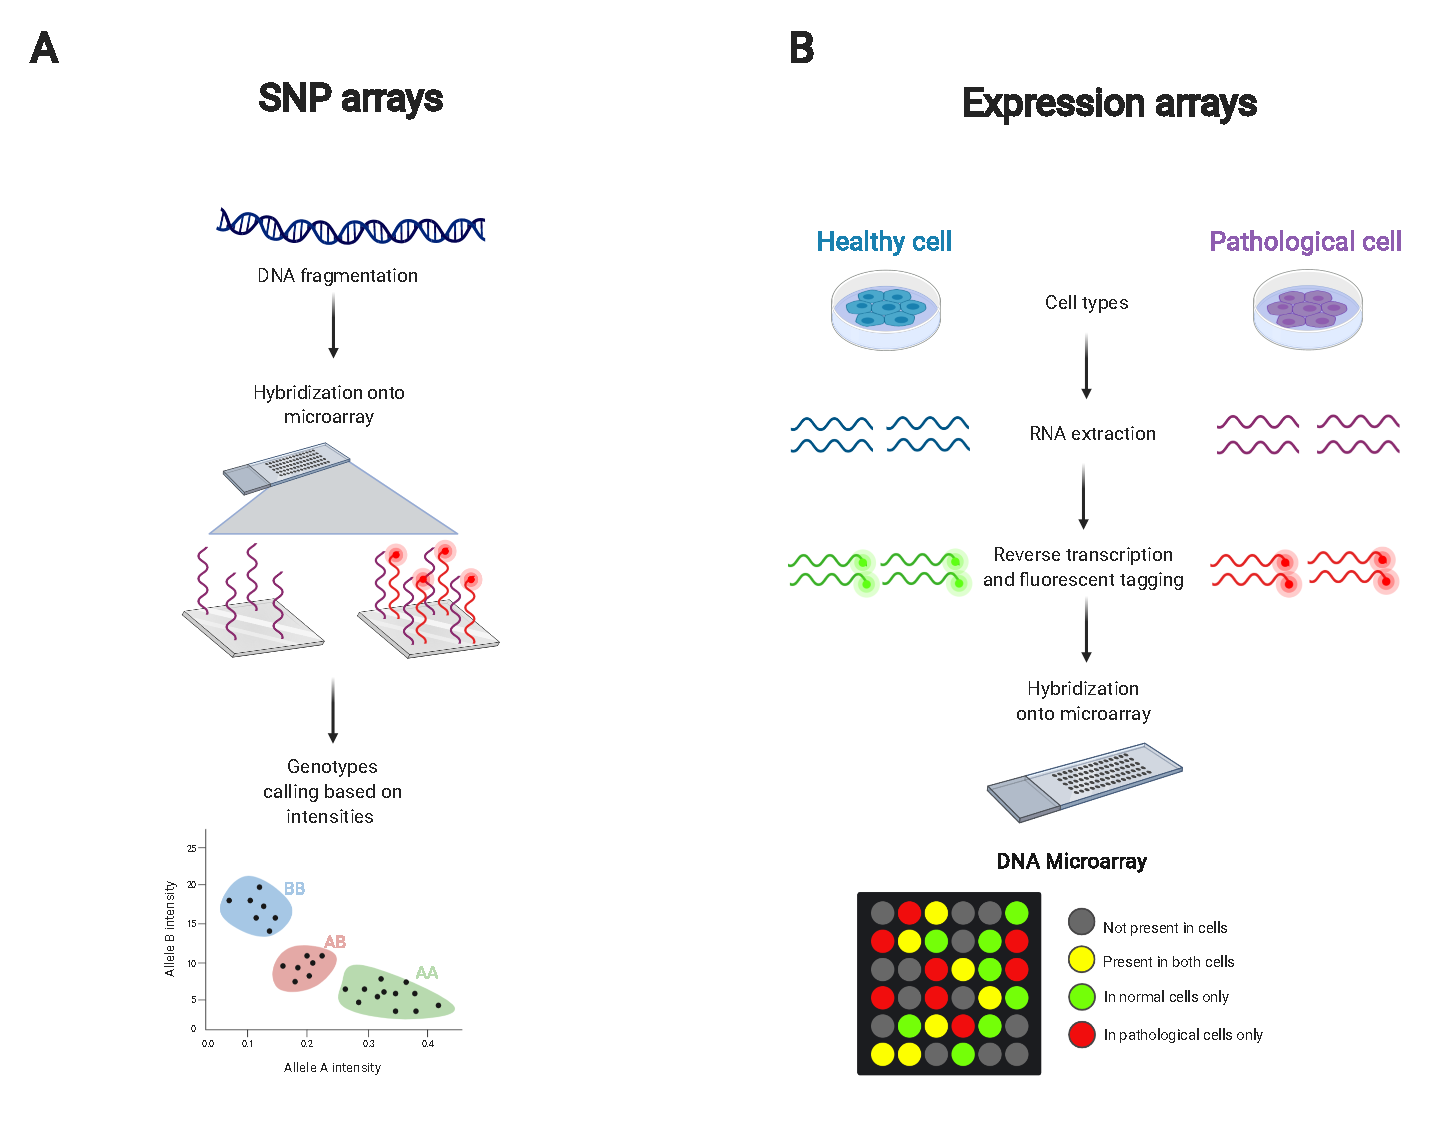
\includegraphics[width=0.9\textwidth]{Figures/Intro/arrays.pdf}
    \caption[Microarrays]{\textbf{Microarrays}. A) \gls*{SNP} arrays: fragmented \gls*{DNA} sequences bind to designed probes on the microarray, which generates an intensity signal that varies depending on the allele carried by the \gls*{DNA} sequences. B) Expression arrays: tagged complementary \gls*{DNA}, reverse-transcribed from \gls{mRNAs} molecules, bind to gene-specific probes, which generates a fluorescence signal used to compare expression levels in different cell conditions. Created with \href{https://biorender.com/}{BioRender.com}}
    \label{fig:intro_arrays}
\end{figure}
In order to study genomic variations across the genome, specific microarrays were developed, the genotyping or \gls*{SNP}s arrays. Those arrays contain unique probe sequences, targeting specific positions of the genome, which hybridize to single-stranded \gls*{DNA} that has been fragmented. This generates intensities signals varying depending on the allele carried by the \gls*{DNA} sequence binding to each probe. This intensity, indicating the presence or absence of each allele, is then converted into genotypes \cite{Laframboise2009} (See Figure \ref{fig:intro_arrays}A). %The first SNP array developed for commercial purposes was the Affymetrix array that has evolved over time to interrogate from 10,000 to 500,000 SNPs.
The \gls*{SNP} arrays developed for commercial purposes have evolved, interrogating from 10,000 to millions of sites simultaneously in a given individual \cite{Xing2016}. Key produces of these technologies were developed by Affymetrix and Illumina inc. Those arrays have been used so far for different purposes. They allowed the identification of copy number changes or, for arrays with high marker density regions, the detection of \gls{LOH} events by identifying regions without heterozygous positions \cite{Beroukhim2006,Dutt2007}. They have also been used to identify germline variants that associate with a certain disease through \gls{GWAS} \cite{XueyingMao2007}. As illustrated in Figure \ref{fig:intro_gwas}, \gls{GWAS} interrogate millions of positions across the genome by testing their association with
a specific trait, like smoking traits, individually and reveal positions significantly associated with that trait.  
\begin{figure}[H]
    \centering
    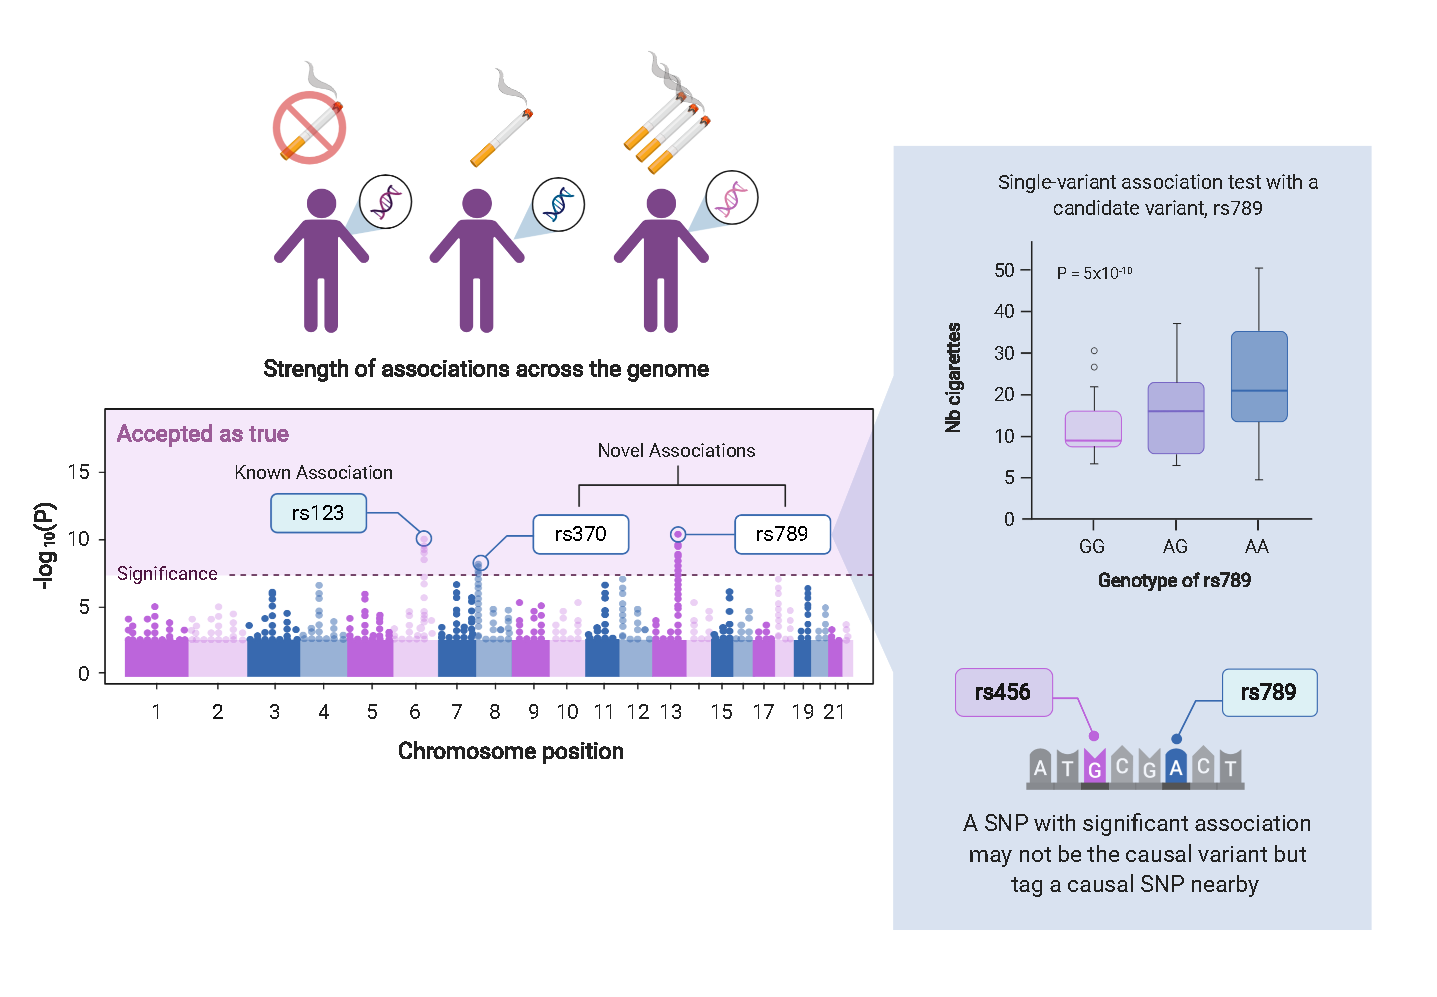
\includegraphics[width=1\textwidth]{Figures/Intro/GWAS.pdf}
    \caption[Genome-wide association studies]{\textbf{Genome-wide association studies}. The figure illustrates a \gls{GWAS} identifying \gls*{SNP}s associated with the number of cigarettes smoked per day. For each position, the association between the variant genotypes and the number of cigarettes per day is tested (rs789 example). The associations \textit{p}-values are represented in a Manhattan plot (left panel). \gls*{SNP}s reaching the genome-wide significance threshold of $5.10^{-8}$ are considered as true associations. Those \gls*{SNP}s do however not always correspond to the causal variant but often tag a nearby \gls*{SNP} in linkage disequilibrium. Created with \href{https://biorender.com/}{BioRender.com}}
    \label{fig:intro_gwas}
\end{figure}
%Today, SNP arrays have the capacity to genotype millions of positions, \textit{e.g.} around five millions markers for the Omni5 array \cite{Xing2016}. 
%Other use of SNP arrays, determining the samples ancestry, which is important in the identification of disease related SNPs. Indeed ....
Although \gls*{SNP}s arrays are limited to the positions assayed, much more positions can be studied based on the arrays. Indeed, \gls*{SNP}s are transmitted to the offspring linked to other close \gls*{SNP}s in blocks called haplotypes. This relationship between \gls*{SNP}s is called \gls{LD}. Knowing the \gls*{SNP}s composition of a haplotype enables to predict the genotype of \gls*{SNP}s that were not assayed by the array by using the information of the assayed positions in the haplotype. Hence, genotyping hundred thousands of \gls*{SNP}s allows actually to impute the genotype of millions of other variants thanks to \gls{LD}. The definition of the haplotypes required though to study such genomic structure in different samples to build a map as reference. Those were the goals of the \gls{HapMap} started in 2002 \cite{Belmont2003,Hapmap_britannica}.

% read this to have ideas on the limitations: https://medium.com/the-gencove-blog/it-is-time-to-replace-genotyping-arrays-with-sequencing-73535efa66ed
%First catalogue of human variation was the HapMap (haplotype map) project. \\

Micro-arrays platforms have also been used to study the other molecular layers like the transcriptome and the methylome. For the analysis of the expression profile, micro-arrays have enabled to measure and compare the expression levels of specific genes in cells under different conditions, \textit{e.g.} diseased versus healthy cells or treated versus non-treated cells. Figure \ref{fig:intro_arrays}B describes the main steps of an expression array experiment. The extracted \gls{mRNAs} molecules from both types of cells, after being reverse-transcribed to \gls{cDNA} and labelled with fluorescent dye, hybridize to the genes specific probes fixed on the array. The array is then scanned using fluorescent imaging \cite{Tarca2006}. The fluorescence amount detected at each probe is proportional to the amount of \gls{mRNAs} in cells. While these measures do not provide absolute quantification of gene expression levels, they enable to compare the expression levels in the different conditions.
%methylation techniques
%Arrays and sequencing methods have allowed to explore the genetic information stored in our DNA. Similar technologies 
Arrays have also been used to study the epigenome by allowing the detection and the analysis of methylation events. The most commonly used methylation arrays are the Illumina arrays \cite{Illumina_Methylation_infinium}. As for the \gls*{SNP}s arrays, probes are designed to target specific loci of the human genome, in this case, \gls{CpG} positions. The number of positions interrogated by such arrays can vary from 25,000 to 850,000 positions depending on the array (\textit{e.g.} Illumina 25K, 450K and 850K arrays). Probes are designed and fixed to the array to bind to both methylated and unmethylated loci (Figure \ref{fig:intro_methylation}). This binding is enabled by a chemical process called bisulfite conversion, which converts unmethylated cytosines to uracil and leave methylated cytosine unchanged. At the hybridization step, a single-based extension is performed with labelled nucleotides, allowing to distinguish for each locus a methylated vs non-methylated signal (Figure \ref{fig:intro_methylation}). The ratio between the two signals at a locus provides a value, called $\beta$ value, which indicates the level of methylation. This value ranges between 0 and 1, 0 corresponding to a non-methylated and 1 a methylated position. 
\begin{figure}[H]
    \centering
    \includegraphics[width=0.8\textwidth]{Figures/Intro/Illumina_methylation2.pdf}
    \caption[The Illumina Infinium methylation assay]{\textbf{The Illumina Infinium methylation assay} (From \cite{Illumina_Methylation_infinium}). This figure represents the probes used for methylation profiling by Illumina. A) Infinium type I probes. Two site-specific probes are found on the array: probes allowing methylated sites with the preserved cytosine to bind (methylated bead M) and probes designed for the unmethylated site with the thymine nucleotide resulting from bisulfite conversion and whole-genome amplification (methylated bead U). B) Infinium type II probes. Only one probe per locus is required to bind to both methylated and unmethylated sites. In that case, single-base extension with labelled nucleotides is used.}
    \label{fig:intro_methylation}
\end{figure}

% read this: https://www.gesundheitsindustrie-bw.de/en/article/news/dna-from-watson-and-crick-to-modern-molecular-biology
\subsubsection*{Next-generation sequencing}
While the \gls*{SNP} arrays enabled to access the genotype information of millions of positions, there was still a need to re-sequence human genomes more efficiently and access the complete \gls*{DNA} sequence to better identify genetic variations. Around 2005, the second generation of sequencing methods called \gls{NGS} has been developed. 
\begin{figure}[H]
    \centering
    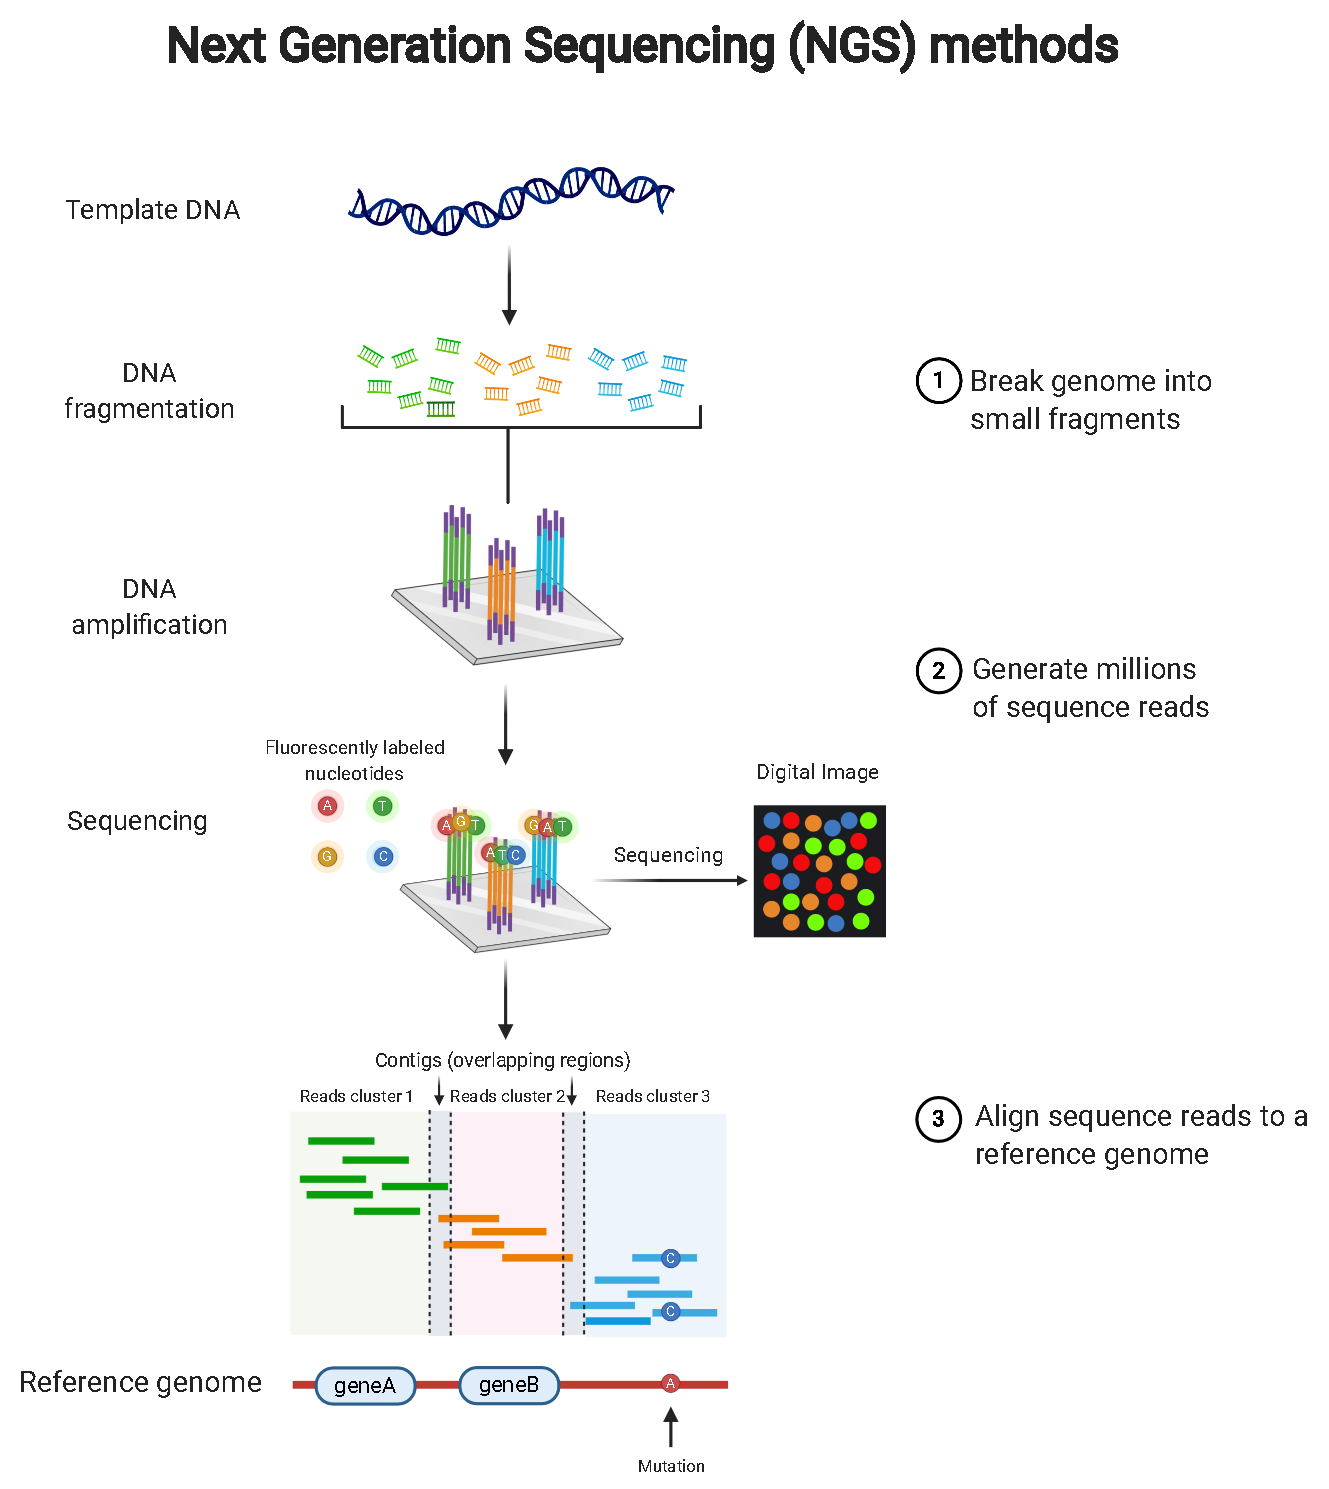
\includegraphics[width=0.8\textwidth]{Figures/Intro/ngs.pdf}
    \caption[Next Generation Sequencing methods]{\textbf{Next Generation Sequencing methods}. The figure describes the \gls{NGS} steps consisting in: i) fragmenting the nucleic acid molecule, ii) amplifying the fragments (using \gls{PCR}), iii) sequencing the resulting copies using single-base extension that adds one after the other labelled nucleotides whose signals are detected using digital imaging. The sequencing reads are then aligned to a reference genome to assemble the reads in a single sequence or to detect mutations across the genome. In the case of \gls*{RNA} sequencing, the reads align to exonic regions of the genes and they are counted to quantify gene expression levels. Created with \href{https://biorender.com/}{BioRender.com}}
    \label{fig:intro_ngs}
\end{figure}
The main change in these new methods in comparison to the first one was the parallelization of the sequencing, which allowed to produce millions of sequences, called reads, at the same time and hence to decrease drastically the time of sequencing as well as its cost \cite{Wetterstrand} (Figure \ref{fig:intro_ngs}). 
\gls{NGS} methods enabled the rapid re-sequencing of different parts and lengths of the genome. The entire genome sequence (except some highly problematic regions) can be accessed with \gls{WGS}. The restricted sequencing of coding regions (exonic regions) can be performed with \gls{WES}. Finally, it is possible to sequence specific regions of the genome, usually genes, using targeted sequencing. 
Based on these techniques, bioinformatics methods have been developed to detect germline as well as somatic variants. They consist in mapping (or aligning) the sequenced reads to a reference genome, and positions that vary from the reference are identified as variations (Figure \ref{fig:intro_ngs}). A mismatch between a sequenced genome and the reference genome is expected around every 1,000 bases. To distinguish somatic from germline mutations, both tumor and normal cells \gls*{DNA} from the same individual have to be sequenced. The tumor \gls*{DNA} is compared to the normal \gls*{DNA} and variations found in the tumor cells only are classified as somatic mutations. Somatic mutations are expected every 1,000,000 bases approximately depending on the cancer type \cite{Alexandrov2013}. 

While the \gls*{DNA} sequencing techniques have been used to detect \gls*{DNA} mutations, they do not explore the expression or methylation layers.
In 2008, the sequencing of the \gls*{RNA} molecule (\gls{RNA-Seq}) had been performed to study expression profiles. In this technique, the \gls{mRNAs} molecules are fragmented and converted to complementary \gls*{DNA} before sequencing, and the resulting reads are aligned to the reference genome \cite{Wang2009}. After the alignment step, the reads can be assigned to genes and the abundance of reads mapped on a gene, quantified using the number of mapped reads, reflects the expression level of the gene (Figure \ref{fig:intro_ngs}). A high read count value indicating that a gene is active and transcribed in that sample. The comparison of the read counts distributions in samples from different conditions, \textit{e.g.} samples with and without disease or diseased samples under different treatment, can be used to identify genes involved in or causing a specific condition. \gls{RNA-Seq} can also be used to identify different transcripts of a gene as well as gene rearrangements like translocations. 

Note that other recent techniques, while not described in the thesis, also exist to access different omics layers. A new sequencing technique has been developed for the analysis of the methylome, the bisulfite sequencing, which in contrast with the methylation arrays, can interrogate millions of \gls{CpG}s positions across the whole genome as well as positions in targeted regions. Also, the study of chromatin accessibility and \gls*{DNA}-binding proteins is possible thanks to \gls{ATAC-seq} and Chromatin immunoprecipitation experiments followed by sequencing (\gls{ChiP-Seq}) respectively \cite{Furey2012,Yan2020}. Finally, while the sequencing methods presented so far process \gls*{DNA} coming from a bulk of cells, single-cell sequencing methods have been developed to perform molecular characterization at the cell level. These methods allow the identification of distinct populations of cells in a tumor and hence the study of tumor heterogeneity and tumor microenvironment \cite{Hwang2018,Finotello2019}.
%The ability to detect the somatic variations in the entire genome of tumor cells have expanded the discovery of driver genes. 
%the 1000 genome dataset that sequenced ... from 26 different populations across the world. This property is used in imputation methods which attempt to estimate the missing genotypes on an array \cite{Marchini2010}. 

The decreasing costs of genotyping and sequencing methods have enabled the establishment of genomics studies involving large cohorts \cite{Wetterstrand}. Sequencing a human genome today costs less than 1,000 dollars using \gls{NGS} methods while it would still cost millions if the Sanger method was chosen. Multiple research groups have coordinated their efforts to create large consortia for that purpose and in many cases have shared the resulting data to the scientific community. The next section provides an overview of some of these initiatives.


\subsection{Large public databases}
%the 1000 genome dataset that sequenced ... from 26 different populations across the world. This property is used in imputation methods which attempt to estimate the missing genotypes on an array \cite{Marchini2010}. 

\subsubsection*{The Cancer Genome Atlas}
\gls{TCGA} is a public database providing access to 10,000 patients whose tumors have undergone multi-omics characterization. The project was launched in 2005 by the \gls{NIH} and aimed at characterizing the genomic alterations underlying several cancer types. For that purpose, multiple omics data were generated \cite{Tomczak2015}. The tumor and normal samples from most of the \gls{TCGA} participants have been sequenced using \gls{WES}. Based on these data, multiple variant callers have been used to catalogue the germline and somatic mutations present in each sample. Genotyping has been performed to analyze copy number variations. The transcriptome of most samples has also been sequenced, using \gls*{RNA} and \gls{miRNAs} sequencing. The methylation profiles of the tumors were explored with the use of 25K or 450K methylation arrays. Finally, protein expression profiling has been performed based on \gls{RPPA}. In addition to the molecular data, clinical and environmental exposures data were collected when possible. The \gls{TCGA} projects also delivered the histopathological images associated to each tumor. Based on these diverse omics and clinical datasets, "marker papers" describing the molecular landscape of each tumor type have been published. While the tissues explored at the beginning of the initiative were limited to lung, brain and ovaries, the \gls{TCGA} data encompasses today molecular data from 33 different cancer types. Those cancer-specific studies led to the identification of genomics alterations causing each cancer type, hence the discovery of new driver genes and potential cancer biomarkers, \textit{i.e.} molecules found in the body as an indicator of a disease or specific condition. Also, cancer subtypes were characterized on the molecular level and subtype-specific alterations were identified, which resulted in new clinical managements of tumors \cite{Weinstein2013}. In parallel to the cancer-specific studies, the \gls{TCGA} research network launched, in 2012, the Pan-Cancer Atlas initiative aiming at exploring the commonalities between cancer types, distinguishing tissue-specific determinants of cancer as well as increasing the statistical power for the identification of genomic alterations \cite{Weinstein2013}. This initiative was completed in 2018 and the data have been released and associated to 27 papers, published in Cell, focusing on three main topics: i) cell-of-origin patterns and cancers subgrouping, ii) oncogenic processes, and iii) signaling pathways involved in cancer \cite{PanCanatlas_site}. 

\subsubsection*{The International Cancer Genome Consortium (ICGC) initiatives}
The \gls{TCGA} studies focused their efforts on the characterization of the cancer exomes. However, exomes represent only 1\% of the human genome and much more can be discovered by exploring the remaining 99\% of the genome. In 2007, the \gls{ICGC} project was launched to study more than 20,000 whole genomes from 50 cancer types having an impact in multiple regions of the world (the 25k initiative).  The international consortium aimed at generating a catalogue of the somatic mutations in those cancer types, sharing the resulting datasets and complementing them with transcriptomic and epigenomic datasets \cite{Hudson2010,Cieslik2020}.
%\subsubsection*{Pan-Cancer Analysis of Whole Genomes (PCAWG)}
Based on the samples included in the \gls{TCGA} and the \gls{ICGC} projects, the \gls{PCAWG} project, an \gls{ICGC} initiative also know as the Pan-Cancer project, has arisen \cite{Campbell2020}. The project relied on more than 2600 samples from 38 different tumor types and aimed at meta-analyzing whole-genome data across cancers along the same lines as the PanCancer Atlas project. The first results from these data have been released in 2020 in a series of publications in Nature \cite{Cieslik2020}. While the \gls{TCGA} initiative enabled the study of the coding regions of the samples, the \gls{PCAWG} project, thanks to the use of whole genome sequences, was designed to explore broader mutational patterns in the coding and non-coding regions, from small to large events like structural variations. For example, chromoplexy and chromothripsis events, which are complex chromosomal rearrangements resulting from catastrophic genomic events, have been observed in more cancers than expected, 17.8\% and 22.3\% of the tumors, respectively \cite{Cieslik2020}. Also, one major result from the \gls{PCAWG} project has been the expansion of the mutational signatures mentioned in section \ref{Intro-biology} \cite{Alexandrov2020}, as well as the discovery of 16 structural variants signatures \cite{Li2020}. 
%The PCAWG genomes were complemented by RNA sequencing data for more than 1000 samples \cite{Cieslik2020}.
%Example of the study of the impact of somatic SVs on genome topology and gene regulation Northcott et al. Nature 2014. 
%Ghavi-Helm et al. Nat Genet 2019: SVs 

% germline
\subsubsection*{UKbiobank}
The previously described projects mainly targeted the somatic landscape of genomes. Other large projects have enabled the research community to explore the germline component of human disease. The largest public dataset, focusing on germline genetics, has been generated by the UKbiobank project, which started in 2010 in the UK. This project gathered data from a population-based cohort of around 500,000 participants between 40 and 69 \cite{Bahcall2018} and had as main objective to improve our understand of the interaction between genetics and multiple human diseases. For that purpose, all participants were genotyped. Besides, multiple other biological samples, like urine, blood and saliva as well as physical measures, \textit{e.g.} brain \gls{MRI}, heart and eye measurements, were collected. It is a prospective cohort; participants are followed up and are linked to electronic health records \cite{Bycroft2018}. The genotyping data of the full cohort were released in 2017. Based on this dataset and the large panel of phenotypes, a multitude of \gls{GWAS} studies related to human diseases have been performed and their resulting summary statistics were made available. In 2019, around 100 \gls{GWAS} studies resulting from the UKbiobank data were available on the \gls{GWAS} catalogue, which provides curated \gls{GWAS} summary statistics results \cite{Buniello2019}. The follow-up of the patients has established that, in 2018, 79,000 of the participants were diagnosed with cancer \cite{Bycroft2018}, which means that cancer-related traits can also be studied using this dataset. After the release of the genotyped and imputed data, \gls{WES} and \gls{WGS} sequencing of the samples have been initiated. Part of the exome data, around 50,000 exomes, have already been released and about 200,000 exomes should be expected by the end of 2020. These data foreshadow future key findings in genomics, a better understanding of molecular and phenotypic interactions and probably an improvement of the translation of those findings in the clinic.% Similarly to the UKbiobank projects, multiple national genomics projects have started worldwide. In France, for example, in the context of the "France médecine génomique 2025" project, two sequencing plateforms were launched in 2017 and the sequencing of around 40,000 genomes is expected every year \cite{France_medecine_genomique}. 


\subsubsection*{Data sharing}
With the increasing number of genomics studies, public repositories, like the \gls{dbGAP}, the \gls{EGA} or \gls{GEO}, have been established to store petabytes of genomics data that can be accessed by the research community. In addition, large projects, like the \gls{TCGA} and \gls{ICGC}, have worked on solutions to improve data storage and accessibility.  %For example, all the \gls{TCGA} data have generated ... terabytes and the genomes sequenced through the \gls{PCAWG} project around 800 terabytes of data. 
One of the goals of those projects was to promote open-access data and the development of tools to foster the reuse of the data by the research community \cite{Weinstein2013,Hudson2010}. In 2010, the \gls{TCGA} provided the data in open access for the first time \cite{TCGA_milestones} and updated and extended the content of the open access data over the years. In 2016, the \gls{GDC} was launched by the \gls{NCI} to store all the \gls{TCGA} data \cite{Jensen2017}. For each omics, the data are categorized by levels: low-level data (raw and unnormalized data) that generally enable individuals re-identification are under controlled access, while higher-level data (processed data, clinical data) that do not permit re-identifiability are available without any requirement. In addition to providing the data storage, the \gls{GDC} also aimed at harmonizing and sharing the bioinformatics pipelines used to process the data \cite{Jensen2017,Gao2019}. The processed data resulting from the PanCancer Atlas papers are also available via the \gls{NIH} \gls{GDC} website \cite{PanCancerAtlas_data} and allow researchers to explore broader genomic features like immune variables \cite{Thorsson2018} or biological pathway measures \cite{Knijnenburg2018}.
Also, cloud computing solutions have been developed to facilitate the analyses of large public genomic datasets while avoiding the download and duplication of the data. The \gls{TCGA} and \gls{ICGC} data are available and can be analyzed on the cloud, for example via the \gls{CGC} \cite{Lau2017} or the \gls{ISB-CGC} \cite{Reynolds2017}. Also, the \gls{ICGC} consortium, to process the \gls{PCAWG} data, has developed a computational tool, Butler, which simplifies genomic analyses that have to be run on clouds environments (academic or commercial) \cite{Yakneen2020}.  \newline

In the past decades, the development of genomics technologies and the implementation of large consortia have enabled to characterize human cancers on the molecular level. The understanding of cancer causes and the biological mechanisms underlying tumor development has been improved. Also, due to the identification of correlations between molecular events and patient's prognosis and response to treatments, molecular studies have impacted the way that tumors are classified and managed in the clinic. 

\begin{comment}
Use of reproducible bioinformatics pipeline (e.g nextflow, give versions, github use, notebooks, docker), cloud computing
Example of data sharing \cite{Phillips2020}
Paper on genomic data sharing in europe: \cite{Saunders2019} 
use citations from \cite{Langmead2018}
\end{comment}
